%% ======================================================================
%% 04b_dynamics.tex -- 3. Modelo (parte 2): dinamica de la base, del modulo aereo y de la bola; identificacion
%% ======================================================================
\subsection{Dinámica de la base móvil}
\label{sec:basedyn}

\paragraph{Ecuaciones de movimiento}
Al aplicar el principio de Lagrange--d'Alembert a la base con la restricción \eqref{eq:pfaff} \cite{fierro1997,siciliano2009}, con el centro de masa a una distancia $x_G$ por delante del eje, se obtiene, en $\{B\}$,
\begin{align}
  M_{\mathrm{eq}}\,\dot v-M x_G\,\omega^2&=\frac{\tau_R+\tau_L}{r}+M g^{B}_x-C_{rr}Mg\cos\beta\,\operatorname{sign}v, \label{eq:basev}\\
  I_{\mathrm{eq}}\,\dot\omega+M x_G\,v\,\omega&=\frac{b}{2r}(\tau_R-\tau_L)+M x_G\,g^{B}_y-\tau_{\mathrm{scrub}}, \label{eq:basew}
\end{align}
donde $M_{\mathrm{eq}}=M+2J_w/r^2$, $I_{\mathrm{eq}}=I_G+Mx_G^2+J_wb^2/(2r^2)$, $J_w$ es la inercia de la rueda incluida la inercia reflejada del rotor, $I_G$ es la inercia de guiñada respecto al centro de masa, $g^{B}_{x,y}$ son las componentes \eqref{eq:gB} de la gravedad y $\tau_{\mathrm{scrub}}$ es la pequeña fricción lateral de las ruedas omnidireccionales. La fuerza lateral de restricción en el eje cierra el sistema. Cada motor TorqueNADO, accionado por el puente H con ciclo de trabajo $u_i\in[-1,1]$ y despreciando la inductancia de armadura, obedece la ley par--velocidad promediada
\begin{equation}
  \tau_i=\tau_s\Big(u_i-\frac{\omega_i}{\omega_0}\Big),\qquad \tau_s=\frac{k_tV_b}{R_a}=\SI{4.94}{\newton\metre},\quad \omega_0=\frac{V_b}{k_e}=\SI{10.5}{\radian\per\second},
  \label{eq:motor}
\end{equation}
con los valores de la hoja de datos en el eje de salida \cite{pitsco_torquenado}. En línea recta a velocidad constante, \eqref{eq:basev} y \eqref{eq:motor} dan la velocidad estacionaria en una pendiente $\beta$:
\begin{equation}
  v_{ss}(u,\beta)=r\omega_0\Big[u-\frac{rMg(\sin\beta+C_{rr}\cos\beta)}{2\tau_s}\Big].
  \label{eq:vss}
\end{equation}
Con el ciclo de trabajo de 15\% usado en las pruebas integradas y la masa medida ($M=\SI{10.4}{\kilo\gram}$), \eqref{eq:vss} predice \SI{0.072}{\metre\per\second} en llano, de acuerdo con los 0,06--\SI{0.08}{\metre\per\second} leídos en la telemetría de LabVIEW, y \SI{0.027}{\metre\per\second} en la rampa de \SI{10}{\degree}. En una pendiente de \SI{20}{\degree} el par de carga llega al 18,4\% del de arranque, por encima del ciclo de trabajo del 15\%, de modo que la base no sube sin aumentar $u$ (Fig.~\ref{fig:base}a). La velocidad máxima en vacío es $r\omega_0=\SI{0.52}{\metre\per\second}$. La aceleración inicial que produce un escalón de ciclo de trabajo $u$ está acotada por $a_0\le 2\tau_su/(Mr)=\SI{2.9}{\metre\per\second\squared}$ para $u=0.15$ (la cota se alcanza cuando la inercia reflejada del rotor es despreciable); este valor es del mismo orden que el límite de vuelco que se deduce a continuación (y supera el de la rampa de \SI{10}{\degree}), y por eso las referencias de la base deben seguir rampas.

\paragraph{Límites de vuelco y de tracción}
Considérese el robot subiendo una pendiente $\beta$ con aceleración $a$ hacia adelante. Tomando momentos de la gravedad y de las fuerzas de d'Alembert respecto a la línea de contacto de las ruedas motrices (traseras), la base no vuelca hacia atrás mientras
\begin{equation}
  a< a_{\max}(\beta)=g\Big(\frac{x_G}{h_G}\cos\beta-\sin\beta\Big),\qquad\text{es decir,}\qquad \tan\beta<\frac{x_G}{h_G}\ \ \text{para }a=0 .
  \label{eq:tip}
\end{equation}
Como el octocóptero se nivela solo, su centro de masa permanece en la vertical de la rótula; al repetir el balance de momentos con su CM en $\vect p_J+h_c\vect z_W$ se ve que $h_c$ se cancela, de modo que, para la condición estática, el módulo aéreo actúa como una masa puntual en la rótula. Las pendientes de vuelco estático se midieron el 23/11 con el robot completo (\SI{10.4}{\kilo\gram}, con todas las baterías y el módulo trabado), inclinándolo a mano sobre cada eje hasta el punto de equilibrio y leyendo el ángulo con un inclinómetro: \SI{21.5}{\degree} hacia atrás, que equivale a subir de frente, y \SI{30.5}{\degree} hacia adelante, que equivale a bajar de frente. De ellas, con $L=\SI{0.22}{\metre}$, resultan $x_G=\SI{88}{\milli\metre}$ y $h_G=\SI{224}{\milli\metre}$. Conviene notar un matiz geométrico: al inclinar el robot sobre suelo plano pivotando sobre ruedas de radio $r=\SI{49.3}{\milli\metre}$, la fórmula $L/(\tan\theta_A+\tan\theta_B)$ da la altura sobre el eje de las ruedas ($h_a=\SI{224}{\milli\metre}$, es decir, $h_a+r=\SI{273}{\milli\metre}$ sobre el suelo con el módulo trabado); al destrabar el módulo para que se nivele en la rótula, la contribución de $h_c$ desaparece y la altura efectiva baja en $(m/M)h_c=\SI{44}{\milli\metre}$ hasta \SI{229}{\milli\metre}. Como ambos efectos ($+r$ y $-mh_c/M$) casi se cancelan, el valor $h_G=\SI{224}{\milli\metre}$ usado en el modelo de módulo nivelado difiere solo \SI{5}{\milli\metre} (un 2\%). Esto confirma la posición longitudinal del CAD (\SI{81}{\milli\metre}) y descarta la de un ensayo anterior (\SI{180}{\milli\metre}). El ángulo de vuelco lateral es $\arctan(b/2h_G)=\SI{40.3}{\degree}$. En la rampa de \SI{10}{\degree} quedan \SI{11.5}{\degree} de margen al subir y \SI{20.5}{\degree} al bajar. Con el módulo en la rótula, el margen de aceleración \eqref{eq:tip} es \SI{3.9}{\metre\per\second\squared} en llano, \SI{2.1}{\metre\per\second\squared} en la rampa de \SI{10}{\degree} y solo \SI{0.26}{\metre\per\second\squared} en una pendiente de \SI{20}{\degree} (Fig.~\ref{fig:base}b). Con los rotores sin empuje, una pendiente de \SI{20}{\degree} queda en el límite de estabilidad estática; los ensayos del curso se limitan a \SI{10}{\degree}. El coeficiente de fricción que necesitan las ruedas motrices, $\mu=Mg(\sin\beta+C_{rr}\cos\beta)/N_r$, con la fuerza normal trasera $N_r=Mg[(L-x_G)\cos\beta+h_G\sin\beta]/L$, es 0,25 en \SI{10}{\degree} y 0,40 en \SI{20}{\degree}, por debajo de los valores típicos de caucho sobre madera contrachapada (0,5--0,8), así que, sin empuje, la tracción no es el límite activo.

\begin{figure}[!htbp]
  \centering
  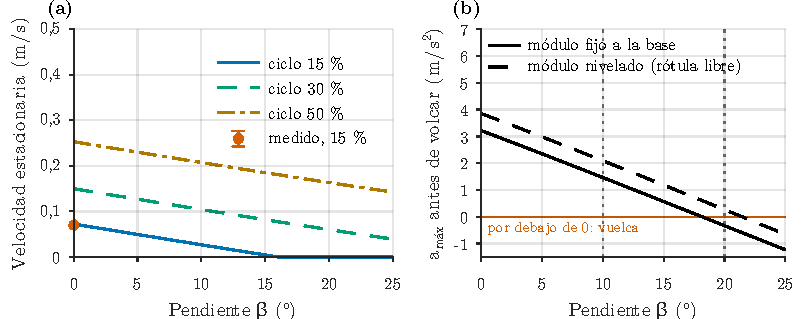
\includegraphics{figures/fig_base_limits.pdf}
  \caption{Base móvil. (a) Velocidad estacionaria frente a la pendiente según \eqref{eq:vss} para tres ciclos de trabajo y velocidad medida al 15\% en llano. (b) Margen de aceleración longitudinal antes de volcar hacia atrás \eqref{eq:tip} con el módulo en la rótula, calibrado con la pendiente de vuelco medida (punto).}
  \label{fig:base}
\end{figure}

\subsection{Dinámica del módulo aéreo}
\label{sec:aerial}

\paragraph{Modelo de rotor y asignación de control}
Cada rotor produce un empuje $F_i$ según $\vect z_D$ y un par de reacción $-c_Qs_iF_i$ alrededor de $\vect z_D$, donde $s_i=+1$ para los rotores antihorarios (vistos desde arriba). Con las posiciones de los rotores $\vect r_i=[x_i,y_i,h_r]\T$ de la Tabla~\ref{tab:params}, el empuje colectivo y los pares en ejes cuerpo son
\begin{equation}
  \begin{bmatrix}T\\ \tau_x\\ \tau_y\\ \tau_z\end{bmatrix}=\underbrace{\begin{bmatrix}\vect 1\T\\ \vect y\T\\ -\vect x\T\\ -c_Q\vect s\T\end{bmatrix}}_{\vect B\in\mathbb R^{4\times8}}\vect F,
  \qquad \vect B\vect B\T=\diag\big(8,\ 4L_r^2,\ 4L_r^2,\ 8c_Q^2\big),
  \label{eq:alloc}
\end{equation}
porque $\sum x_i=\sum y_i=\sum s_i=\sum x_iy_i=\sum s_ix_i=\sum s_iy_i=0$ y $\sum x_i^2=\sum y_i^2=4L_r^2$ para la geometría del octocóptero (la altura de los brazos $h_r$ no contribuye porque el empuje es paralelo a $\vect z_D$). Los cuatro canales son, por tanto, ortogonales y la asignación de norma mínima es explícita:
\begin{equation}
  \vect F=\vect B\T(\vect B\vect B\T)^{-1}\vect w=\frac{T}{8}\vect 1+\frac{\vect y\,\tau_x-\vect x\,\tau_y}{4L_r^2}-\frac{\vect s\,\tau_z}{8c_Q},\qquad \vect w=[T,\tau_x,\tau_y,\tau_z]\T .
  \label{eq:alloc_inv}
\end{equation}
El firmware implementa exactamente \eqref{eq:alloc_inv} \cite{johansen2013}: el colectivo fija la fuerza base $F_0=T/8$, se suman los incrementos de alabeo y cabeceo, y el incremento de guiñada se suma según la fila de guiñada proyectada en el espacio nulo de las otras tres (que, por la ortogonalidad anterior, es la propia fila de guiñada). Cuando un incremento llevaría un rotor fuera de $[F_{\min},F_{\max}]$ (\SIrange{1180}{2000}{\micro\second}), se escalan primero el alabeo y el cabeceo y después la guiñada. Para un par de cabeceo puro saturan primero los rotores del eje $x$ ($|x_i|=L_r$), de modo que el par alcanzable es
\begin{equation}
  |\tau_y|_{\max}=4L_r\,\min\{F_{\max}-F_0,\ F_0-F_{\min}\},
  \label{eq:taumax}
\end{equation}
que, con el mapa del firmware, vale \SI{3.2}{\newton\metre} con un colectivo de \SI{1750}{\micro\second} y \SI{2.4}{\newton\metre} con \SI{1816}{\micro\second}, muy por encima de los pares que pide el vuelo estacionario (Sección~\ref{sec:authority}). El firmware convierte cada fuerza en un pulso invirtiendo el mapa $F=k_F\big((u-u_0)/\SI{860}{\micro\second}\big)^n$ con $k_F=\SI{5.40}{\newton}$; si la ganancia real es $k_F'$, cada par que produce el controlador queda multiplicado por la razón de ganancias de empuje $k_T=k_F'/k_F$, que identifica la Sección~\ref{sec:ident}.

\paragraph{Ecuaciones de Newton--Euler alrededor del pivote móvil}
El conjunto que rota (masa $m$, inercia $\vect J$ respecto a la rótula, centro de masa en $\vect r_c=[\delta_x,\delta_y,h_c]\T$ en $\{D\}$) gira alrededor del centro de la rótula, un punto fijo en el cuerpo al que la base y la guía imponen la aceleración $\vect a_J$ \eqref{eq:aJ}. Para un punto fijo en un cuerpo rígido, el momento angular respecto a él es $\vect J\vect\omega_D$, y su derivada inercial es igual al momento externo menos $m\,\vect r_c\times\vect a_J$ \cite{ginsberg1998}. En componentes de $\{D\}$:
\begin{equation}
  \vect J\dot{\vect\omega}_D+\vect\omega_D\times\vect J\vect\omega_D=
  \underbrace{\sum_{i=1}^{8}\vect r_i\times F_i\ez-\sum_{i=1}^{8}c_Qs_iF_i\ez}_{[\tau_x,\ \tau_y,\ \tau_z]\T}
  +\,m\,\vect r_c\times\Rot_{WD}\T\big(\vect g_W-\vect a_J\big)-\vect\tau_f ,
  \label{eq:euler}
\end{equation}
con $\vect g_W=[0,0,-g]\T$ y $\vect\tau_f$ la fricción de la rótula. El tercer término contiene los tres acoplamientos que dominan el comportamiento del módulo. Linealizando alrededor del vuelo estacionario nivelado (verificado simbólicamente, \ref{app:derivations}):
\begin{align}
  J_x\ddot\phi&=\tau_x+m(g+a_{J,z})h_c\,\phi+m h_c\,a_{J,y}-m g\,\delta_y, \label{eq:rolllin}\\
  J_y\ddot\theta&=\tau_y+m(g+a_{J,z})h_c\,\theta-m h_c\,a_{J,x}+m g\,\delta_x, \label{eq:pitchlin}
\end{align}
con $\vect a_J$ en componentes de $\{D\}$. (i) Como $h_c>0$, el módulo es un péndulo invertido sobre la rótula, con polos en lazo abierto $\pm p$, $p=\sqrt{mgh_c/J_y}=\SI{6.1}{\radian\per\second}$ para $h_c=\SI{0.14}{\metre}$ (tiempo de duplicación \SI{0.11}{\second}). (ii) Una aceleración horizontal de la base produce el par $\mp mh_ca_J$: la parte superior del módulo se queda atrás respecto a la rótula, que es el camino principal de perturbación de la base al octocóptero. (iii) Una excentricidad horizontal $\delta$ del centro de masa produce un par constante $mg\delta$ que el controlador debe sostener de forma permanente. La aceleración vertical de la rótula modula paramétricamente la rigidez del péndulo.

A lo largo de la guía (eje $\vect z_B$), el carro y el módulo obedecen
\begin{equation}
  (m+m_c)\ddot d=T\,\vect z_D\!\cdot\!\vect z_B-(m+m_c)\big(g\cos\beta+\vect a_B\!\cdot\!\vect z_B\big)-F_g(\dot d)+F_{\mathrm{stop}},
  \label{eq:guide}
\end{equation}
de modo que el módulo despega cuando $T>(m+m_c)g\cos\beta+F_{g,\mathrm{static}}$. Mientras $T$ es menor, el módulo apoya en el tope inferior y su peso menos $T$ se transmite a la base; esta es la descarga que se aprovecha en la rampa (Sección~\ref{sec:porquedron}).

\paragraph{Potencia en vuelo estacionario}
Por la teoría de cantidad de movimiento \cite{leishman2006}, el empuje de vuelo estacionario por rotor, $T/8=\SI{4.41}{\newton}$, a través del disco de una hélice de 9,4 pulgadas induce una velocidad $v_h=\sqrt{T/(16\rho A)}=\SI{6.4}{\metre\per\second}$ y requiere una potencia ideal $Tv_h/8=\SI{28}{\watt}$ por rotor. Con una figura de mérito de 0,5 y una eficiencia motor--ESC de 0,8, los ocho rotores consumen unos \SI{570}{\watt}; la tabla del A2212 con hélice 9450, escalada a \SI{3.6}{\kilo\gram}, da \SI{500}{\watt}. Son 22--\SI{25}{\ampere} por rama con fusible, y la potencia crece como $T^{3/2}$, así que cada aumento de colectivo para compensar la caída de tensión cuesta corriente. Por eso el firmware limita a \SI{20}{\second} la operación por encima de \SI{1850}{\micro\second} (fusibles de \SI{30}{\ampere}), y por eso se mantuvo la holgura de \SI{29}{\milli\metre} entre puntas de hélice con $L_r=\SI{0.350}{\metre}$. La Sección~\ref{sec:bateria} convierte estas cifras en margen de empuje y autonomía.

\subsection{Identificación del módulo aéreo con telemetría de vuelo estacionario}
\label{sec:ident}

\paragraph{Ganancia de empuje}
En el despegue, \eqref{eq:guide} da $8k_F'\big((u-u_0)/860\big)^n=(m+m_c)g+F_{g,\mathrm{static}}$. El despegue ocurrió entre \SI{1725}{\micro\second} y \SI{1775}{\micro\second} con las LiPo cargadas, a 12,4\,V en reposo al iniciar la sesión (Sección~\ref{sec:flights}); despreciando la fricción de la guía se obtienen las cotas inferiores $k_F'=$ \SIrange{7.17}{8.18}{\newton}, de modo que la razón de ganancias de empuje es $k_T=1.33$--1,52 (Fig.~\ref{fig:ident}b). El mapa del firmware, y el modelo de Isaac Lab construido sobre él, predecían el vuelo estacionario en \SI{1899}{\micro\second}; una auditoría de potencia independiente, basada en los datos del motor y la hélice, predijo \SI{1770}{\micro\second}, dentro de la banda medida, aunque para una masa de \SI{3.10}{\kilo\gram} y no de \SI{3.6}{\kilo\gram}.

\paragraph{Centro de masa}
Durante el vuelo estacionario cuasiestático ($\dot{\vect\omega}_D\approx\vect 0$, integradores asentados, $T\approx(m+m_c)g$), \eqref{eq:rolllin}--\eqref{eq:pitchlin} se reducen a balances de momentos. Al dividir por el colectivo se elimina la ganancia desconocida $k_F'$ y queda la posición del centro de empuje,
\begin{equation}
  x_{cp}=\frac{\sum_i x_iF_i}{\sum_iF_i}=c\,(\delta_x+h_c\sin\theta),\qquad
  y_{cp}=\frac{\sum_i y_iF_i}{\sum_iF_i}=c\,(\delta_y-h_c\sin\phi),
  \label{eq:cop}
\end{equation}
con $c=m/(m+m_c)$, que es lineal en $(\delta_x,\delta_y,h_c)$ y se calcula con las órdenes de motor registradas. Promediando \eqref{eq:cop} en la fase de vuelo estacionario de los siete vuelos que despegaron (muestras con $|p|,|q|<\SI{15}{\degree\per\second}$ por encima de \SI{1650}{\micro\second}) y resolviendo las 14 ecuaciones por mínimos cuadrados se obtiene
\begin{equation}
  \hat\delta_x=9.5\pm1.8\ \mathrm{mm},\qquad \hat\delta_y=1.9\pm1.5\ \mathrm{mm},\qquad \hat h_c=0.14\pm0.06\ \mathrm{m}\quad(\pm1\sigma),
  \label{eq:idres}
\end{equation}
con un residuo de \SI{3.3}{\milli\metre} RMS (Fig.~\ref{fig:ident}a). La estimación de $h_c$ cambia menos que su incertidumbre cuando el exponente del mapa varía entre 1,3 y 1,6 (0,11--\SI{0.14}{\metre}), y es coherente con los \SI{0.10}{\metre} del modelo derivado del CAD. La excentricidad produce un par de gravedad permanente $mg\delta_x=\SI{0.31}{\newton\metre}$ hacia M8.

\begin{figure}[!htbp]
  \centering
  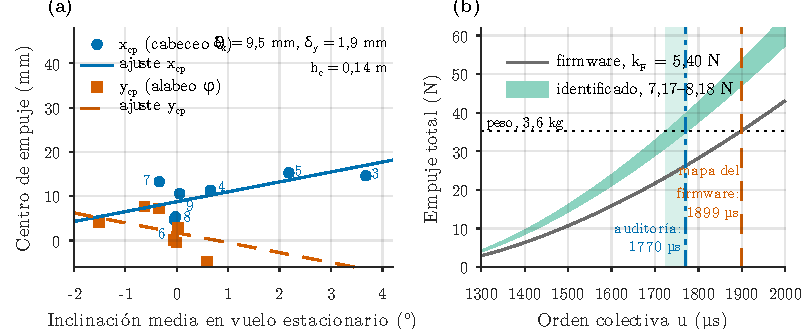
\includegraphics{figures/fig_ident.pdf}
  \caption{Identificación con telemetría de vuelo estacionario. (a) Centro de empuje frente a la inclinación media en los siete vuelos estacionarios (etiquetas: número de vuelo) y ajuste por mínimos cuadrados de \eqref{eq:cop}. (b) Empuje total del mapa del firmware, banda identificada con la condición de despegue, peso del conjunto móvil y predicciones de vuelo estacionario del mapa del firmware y de la auditoría de potencia.}
  \label{fig:ident}
\end{figure}

\subsection{Bola sobre un plato que acelera y rota}
\label{sec:ball}

Sea $\vect\Omega$ la velocidad angular del marco del plato $\{P\}$ y sea $\vect a_G$ la aceleración absoluta de su origen (el centro de la junta universal), ambas expresadas en $\{P\}$. El centro de la bola está en $\vect\rho=[x_b,y_b,\varepsilon]\T$, su velocidad angular absoluta es $\vect\omega_b$, y la rodadura sin deslizamiento (A6) exige que la velocidad del punto de contacto de la bola sea igual a la del punto del plato que toca. Esto da $\dot{\vect\rho}=r_b(\vect\omega_b-\vect\Omega)\times\ez$, es decir, la velocidad angular relativa es $\vect w=\vect\omega_b-\vect\Omega=[-\dot y_b/r_b,\ \dot x_b/r_b,\ w_z]\T$, con un giro libre $w_z$ alrededor de la normal del plato. Escribiendo la ley de Newton para el centro de la bola en el marco que rota y la ley de Euler para la bola respecto a su centro, con la fuerza de contacto aplicada en $-r_b\ez$, y eliminando las fuerzas tangenciales de contacto (\ref{app:derivations}), se obtiene, de forma exacta,
\begin{align}
  \frac{\ddot x_b}{\gamma_b}&=g_x-a_{G,x}-\kappa\dot\Omega_y+\dot\Omega_z\,y_b+(\Omega_y^2+\Omega_z^2)\,x_b-\Omega_x\Omega_y\,y_b \notag\\
   &\quad-\varepsilon\,\Omega_x\Omega_z+(2+\iota)\,\Omega_z\dot y_b+\iota r_b\,\Omega_xw_z, \label{eq:ballx}\\
  \frac{\ddot y_b}{\gamma_b}&=g_y-a_{G,y}+\kappa\dot\Omega_x-\dot\Omega_z\,x_b+(\Omega_x^2+\Omega_z^2)\,y_b-\Omega_x\Omega_y\,x_b \notag\\
   &\quad-\varepsilon\,\Omega_y\Omega_z-(2+\iota)\,\Omega_z\dot x_b+\iota r_b\,\Omega_yw_z, \label{eq:bally}\\
  \dot w_z&=-\dot\Omega_z-\frac{\Omega_x\dot x_b+\Omega_y\dot y_b}{r_b}, \label{eq:spin}
\end{align}
donde $[g_x,g_y,g_z]\T=\Rot_{WP}\T\vect g_W$ es la gravedad en $\{P\}$, $\iota=I_b/(m_br_b^2)$ ($2/5$ para una esfera maciza), $\gamma_b=1/(1+\iota)$, y
\begin{equation}
  \kappa=\varepsilon+\frac{I_b}{m_br_b}=\varepsilon+\iota r_b=\SI{42.3}{\milli\metre}
  \label{eq:kappa}
\end{equation}
es la altura efectiva de la bola sobre el eje de rotación. Las ecuaciones \eqref{eq:ballx}--\eqref{eq:spin} contienen el modelo clásico del \textit{ball and plate} como caso particular con $\vect a_G=\vect 0$, $\Omega_z=0$, $\varepsilon=0$ \cite{awtar2002,hauser1992}; los términos adicionales son la aceleración de arrastre del centro del plato, el término de Euler $\kappa\dot{\vect\Omega}$ debido a la altura de la bola, los términos centrífugo y de Coriolis de la rotación de la base y el acoplamiento del giro propio.

\paragraph{Linealización y funciones de transferencia}
Para ángulos pequeños, $g_x\simeq g\,\Theta_P$ y $g_y\simeq-g\,\Phi_P$; con \eqref{eq:tilt} y la linealización de \eqref{eq:aG}, $a_{G,x}\simeq a_{J,x}+h_P\ddot\theta$ y $a_{G,y}\simeq a_{J,y}-h_P\ddot\phi$, la bola obedece
\begin{align}
  \ddot x_b&=\gamma_b\Big[g(\theta+\alpha_y)-\kappa\,\ddot\alpha_y-(h_P+\kappa)\,\ddot\theta-a_{J,x}\Big], \label{eq:balllinx}\\
  \ddot y_b&=\gamma_b\Big[-g(\phi+\alpha_x)+\kappa\,\ddot\alpha_x+(h_P+\kappa)\,\ddot\phi-a_{J,y}\Big]. \label{eq:balllinly}
\end{align}
Las ecuaciones \eqref{eq:balllinx}--\eqref{eq:balllinly} resumen el acoplamiento de todo el robot: a la bola la mueven la inclinación de los servos (la entrada de control), la actitud residual del octocóptero amplificada por el brazo $h_P+\kappa=\SI{0.146}{\metre}$, y la aceleración de la rótula que produce la base. Con $\alpha_y=K_\alpha u$, las tres funciones de transferencia del eje $x$ son
\begin{equation}
  \frac{X_b}{U}=K_b\,\frac{1-s^2/z_1^2}{s^2},\qquad
  \frac{X_b}{\Theta}=\gamma_b g\,\frac{1-s^2/z_2^2}{s^2},\qquad
  \frac{X_b}{A_{J,x}}=-\frac{\gamma_b}{s^2},
  \label{eq:balltf}
\end{equation}
con la ganancia de planta $K_b=\gamma_bgK_\alpha=\SI{6.0}{\milli\metre\per\second\squared}$ por microsegundo (bola maciza) y los ceros $z_1=\sqrt{g/\kappa}=\SI{15.2}{\radian\per\second}$ y $z_2=\sqrt{g/(h_P+\kappa)}=\SI{8.2}{\radian\per\second}$. Cada par contiene un cero en el semiplano derecho: el camino del servo es de fase no mínima (una inclinación rápida empuja primero la bola en el sentido equivocado, porque la superficie del plato acelera bajo ella), y por encima de $z_2/2\pi=\SI{1.3}{\hertz}$ la aceleración angular del octocóptero perturba la bola más que su inclinación.

\paragraph{Rotación de la base}
Para una base que gira a velocidad constante $\omega$ ($\vect\Omega=\omega\ez$), \eqref{eq:ballx}--\eqref{eq:bally} añaden la rigidez negativa $\gamma_b\omega^2$ y el acoplamiento giroscópico $\gamma_b(2+\iota)\omega$ entre los ejes. Incluso para un giro más rápido que cualquier prueba ($\omega=\SI{0.53}{\radian\per\second}$, ruedas a $\pm\SI{0.10}{\metre\per\second}$), la rigidez negativa es \SI{0.20}{\per\second\squared}, menos del 10\% de la rigidez $K_bk_p\approx\SI{2}{\per\second\squared}$ que aporta el controlador de la bola (Sección~\ref{sec:ballcontrol}).
